
\documentclass{beamer}

\usetheme{Warsaw}
\usepackage{xcolor}
\usepackage{minted}
\usepackage{pgfplots}
\usepackage{amsfonts}
\usepackage{svg}

\usepackage{tikz}
\usetikzlibrary{mindmap,trees}
\usetikzlibrary{calc}
\usepackage{relsize}
\usepackage{scalefnt}


\tikzset{fontscale/.style = {font=\relsize{#1}}
    }

\definecolor{monokai_gray}{RGB}{39,40,34}
\definecolor{monokai_pink}{RGB}{249,38,114}
\definecolor{monokai_blue}{RGB}{102,217,239}
\definecolor{monokai_green}{RGB}{166,226,46}
\definecolor{monokai_orange}{RGB}{253,151,31}
\definecolor{monokai_bg}{RGB}{39,40,34}
\definecolor{monokai_red}{RGB}{247, 0, 94}
\definecolor{monokai_light_gray}{RGB}{98, 95, 75}
\definecolor{monokai_white}{RGB}{246, 247, 238}
\definecolor{monokai_yellow}{RGB}{224, 215, 90}
% \definecolor{monokai_bg}{rgb}{0.1529,0.1569,0.1333}
% \definecolor{monokai_bg}{rgb}{0.1529,0.1569,0.1333}

\usepackage{amsmath}
\DeclareMathOperator*{\argmax}{arg\,max}
\DeclareMathOperator*{\argmin}{arg\,min}

\usepackage[absolute,overlay]{textpos}

\usepackage{tikz}



\usemintedstyle{monokai}

\setbeamercolor{normal text}{fg=white,bg=monokai_gray}
\setbeamercolor{structure}{fg=white}

%\setbeamercolor{alerted text}{parent=structure,bg=monokai_gray!95}

\setbeamercolor{item projected}{use=item,fg=black,bg=item.fg!35}

\setbeamercolor*{palette primary}{use=structure,fg=structure.fg}
\setbeamercolor*{palette secondary}{use=structure,fg=structure.fg!95!black}
\setbeamercolor*{palette tertiary}{use=structure,fg=structure.fg!90!black}
\setbeamercolor*{palette quaternary}{use=structure,fg=structure.fg!95!black,bg=black!80}

\setbeamercolor*{framesubtitle}{fg=white}

\setbeamercolor*{block title}{parent=structure,bg=monokai_gray!95}
%\setbeamercolor*{block body}{fg=black,bg=monokai_blue!30}
\setbeamercolor*{block title alerted}{parent=structure,bg=monokai_gray!95}
\setbeamercolor*{block title example}{parent=structure,bg=monokai_gray!95}


\setbeamertemplate{headline}{}
\setbeamertemplate{footline}[frame number]
\setbeamertemplate{section in toc}[ball unnumbered]



%\beamertemplatenavigationsymbolsempty






\def\layersep{2.5cm}


\usepackage{minted}

\newminted{python}{fontsize=\scriptsize, 
                   linenos,
                    numbersep=8pt,
                   autogobble,
                   %fontsize=\small,%baselinestretch=1,
                   frame=lines,
                   bgcolor=bg} 

\newminted{cpp}{fontsize=\scriptsize, 
                   linenos,
                   numbersep=8pt,
                   autogobble,
                   %fontsize=\small,%baselinestretch=1,
                   frame=lines,
                   bgcolor=bg} 
\newminted{r}{fontsize=\scriptsize, 
                   linenos,
                   numbersep=8pt,
                   autogobble,
                   %fontsize=\small,%baselinestretch=1,
                   frame=lines,
                   bgcolor=bg} 
\newminted{julia}{fontsize=\scriptsize, 
                   linenos,
                   numbersep=8pt,
                   autogobble,
                   %fontsize=\small,%baselinestretch=1,
                   frame=lines,
                   bgcolor=bg} 

\newmint[lcpp]{cpp}{}
\newmint[lpython]{python}{}

%Information to be included in the title page:
\title{Multiple Things}
\subtitle{a bit of everything}
\author{Thorsten Beier}
 

\begin{document}


\begin{frame}[label=current]
\titlepage
\end{frame}

\begin{frame}
  \visible<+->{Outline}
  \begin{itemize}
        \item<+->Deep Learning / Neural Network Frameworks
        \begin{itemize}
            \item<+-> Autoencoders
            \item<+-> Variational Autoencoders
            \item<+-> Convolutional Autoencoders
            \item<+-> PyTorch
            \item<+-> Inferno
        \end{itemize}
        \item<+->Modern C++
        \begin{itemize}
            \item<+-> Why
            \item<+-> C++, on language to rule them all
            \item<+-> Ultra Rapid Development with C++
        \end{itemize}     
        \item<+-> Discrete Optimization
        \begin{itemize}
            \item<+-> Energy Minimization
            \item<+-> Graphical Models
        \end{itemize}        
  \end{itemize}
\end{frame}



\setbeamercolor{framesource}{fg=gray}
\setbeamerfont{framesource}{size=\tiny}

\newcommand{\source}[1]{\begin{textblock*}{12cm}(0.0cm, 8.0cm)
    \begin{beamercolorbox}[ht=0.5cm,right]{framesource}
        \usebeamerfont{framesource}\usebeamercolor[fg]{framesource} Source: {#1}
    \end{beamercolorbox}
\end{textblock*}}


\newcommand{\imgsource}[1]{\begin{textblock*}{12cm}(0.0cm, 8.0cm)
    \begin{beamercolorbox}[ht=0.5cm,right]{framesource}
        \usebeamerfont{framesource}\usebeamercolor[fg]{framesource} Image Source: {#1}
    \end{beamercolorbox}
\end{textblock*}}


\newcommand{\moreinfo}[1]{\begin{textblock*}{12cm}(0.0cm, 8.0cm)
    \begin{beamercolorbox}[ht=0.5cm,right]{framesource}
        \usebeamerfont{framesource}\usebeamercolor[fg]{framesource} More Infos: {#1}
    \end{beamercolorbox}
\end{textblock*}}

\newcommand{\tryit}[1]{\begin{textblock*}{12cm}(0.0cm, 8.0cm)
    \begin{beamercolorbox}[ht=0.5cm,right]{framesource}
        \usebeamerfont{framesource}\usebeamercolor[fg]{framesource} Try it out: {#1}
    \end{beamercolorbox}
\end{textblock*}}


\newcommand{\basedon}[1]{\begin{textblock*}{12cm}(0.0cm, 8.0cm)
    \begin{beamercolorbox}[ht=0.5cm,left]{framesource}
        \usebeamerfont{framesource}\usebeamercolor[fg]{framesource} Based On: {#1}
    \end{beamercolorbox}
\end{textblock*}}



\begin{frame}\frametitle{Autoencoders}
\centering
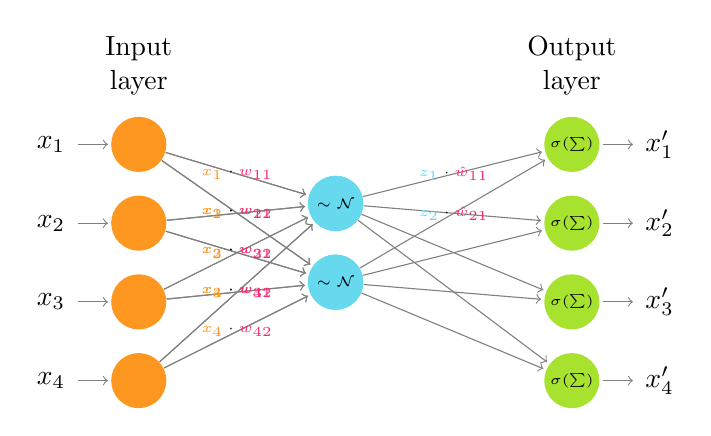
\begin{tikzpicture}[shorten >=1pt,->,draw=black!50, node distance=\layersep]
    \tikzstyle{every pin edge}=[<-,shorten <=1pt]
    \tikzstyle{neuron}=[circle,fill=black!25,minimum size=17pt,inner sep=0pt,minimum size=0.7cm]
    \tikzstyle{input neuron}=[neuron, fill=monokai_orange];
    \tikzstyle{output neuron}=[neuron, fill=monokai_green];
    \tikzstyle{hidden neuron}=[neuron, fill=monokai_blue];
    \tikzstyle{annot} = [text width=4em, text centered]
    \tikzstyle{eln} = [midway, font=\tiny]

    \visible<1-11>{
    \visible<1->{

        % Draw the input layer nodes
        \foreach \name / \x in {1,...,4}
        % This is the same as writing \foreach \name / \x in {1/1,2/2,3/3,4/4}
            \node[input neuron, pin=left: $x_\x$] (I-\name) at (0,-\x) {};

        
        % \node[annot,above of=H-1, node distance=2cm] (hl) { \phantom{Hidden layer}};
        \node[annot, above of=I-1, node distance=1cm] () {Input layer};
        % \node[annot,right of=hl] {Output layer};

    }
    }

    \visible<2-7>
    {
    % Draw the hidden layer nodes
    \foreach \name / \y in {1,...,2 }
        \path[yshift=0.5cm]
            node[hidden neuron,font=\small] (H-\name) at (\layersep,-\y cm - 1.25cm) {};

    }
    \visible<8-11>
    {
    % Draw the hidden layer nodes
    \foreach \name / \y in {1,...,2 }
        \path[yshift=0.5cm]
            node[hidden neuron,font=\small] (H-\name) at (\layersep,-\y cm - 1.25cm) {\tiny$\sigma(\sum)$};

    }
    \visible<12->
    {
    % Draw the hidden layer nodes
    \foreach \name / \y in {1,...,2 }
        \path[yshift=0.5cm]
            node[hidden neuron,font=\small] (H-\name) at (\layersep,-\y cm - 1.25cm) {\tiny$\sim\mathcal{N}$};

    }
    \visible<1-11>{
    % draw the edges
    \visible<3->
    {
        % Connect every node in the input layer with every node in the
        % hidden layer.
        % \foreach \i in {1}
        %     \foreach \j in {1,...,2}
        %         \draw (I-\i) -- (H-\j) node [eln] {$x_\i \cdot w_{\i\j}$};

        \foreach \i in {1,2,3,4}
            \foreach \j in {1,...,2}
                \draw (I-\i) -- (H-\j);% node [eln] {$x_\i \cdot w_{\i\j}$};
    }
    % show the math..
    \visible<4>
    {
        % Connect every node in the input layer with every node in the
        % hidden layer.
        \foreach \i in {1}
            \foreach \j in {1,...,2}
                \draw (I-\i) -- (H-\j) node [eln ] {$\textcolor{monokai_orange}{x_\i}  \cdot \textcolor{monokai_pink}{w_{\i\j}}$};

        % \foreach \i in {2,3,4,5,6}
        %     \foreach \j in {1,...,2}
        %         \draw (I-\i) -- (H-\j);% node [eln] {$x_\i w_{\i\j}$};
    }
    \visible<5>
    {
        % Connect every node in the input layer with every node in the
        % hidden layer.
        \foreach \i in {2}
            \foreach \j in {1,...,2}
                \draw (I-\i) -- (H-\j) node [eln ] {$\textcolor{monokai_orange}{x_\i}  \cdot \textcolor{monokai_pink}{w_{\i\j}}$};

        % \foreach \i in {2,3,4,5,6}
        %     \foreach \j in {1,...,2}
        %         \draw (I-\i) -- (H-\j);% node [eln] {$x_\i w_{\i\j}$};
    }
    \visible<6>
    {
        % Connect every node in the input layer with every node in the
        % hidden layer.
        \foreach \i in {3}
            \foreach \j in {1,...,2}
                \draw (I-\i) -- (H-\j) node [eln ] {$\textcolor{monokai_orange}{x_\i}  \cdot \textcolor{monokai_pink}{w_{\i\j}}$};

        % \foreach \i in {2,3,4,5,6}
        %     \foreach \j in {1,...,2}
        %         \draw (I-\i) -- (H-\j);% node [eln] {$x_\i w_{\i\j}$};
    }
    \visible<7->
    {
        % Connect every node in the input layer with every node in the
        % hidden layer.
        \foreach \i in {4}
            \foreach \j in {1,...,2}
                \draw (I-\i) -- (H-\j) node [eln ] {$\textcolor{monokai_orange}{x_\i}  \cdot \textcolor{monokai_pink}{w_{\i\j}}$};

        % \foreach \i in {2,3,4,5,6}
        %     \foreach \j in {1,...,2}
        %         \draw (I-\i) -- (H-\j);% node [eln] {$x_\i \cdot w_{\i\j}$};
    }

    }

    \visible<9,10, 12>
    {
     

    % Draw the output layer nodes

    \foreach \name / \y in {1,...,4}
        \node[output neuron,pin={[pin edge={->}]right:$x_\y'$}, right of=H-3] (O-\name) at (3,-\y) {\tiny$\sigma(\sum)$};

      
      {
      % Connect every node in the hidden layer with the output layer
      \foreach \i in {1,2}
          \foreach \j in {2,...,4}
              \draw (H-\i) -- (O-\j);
      }
      {
      % Connect every node in the hidden layer with the output layer
      \foreach \i in {1,2}
          \foreach \j in {1}
              \draw (H-\i) -- (O-\j) node [eln ] {$\textcolor{monokai_blue}{z_\i}  \cdot \textcolor{monokai_pink}{\hat{w}_{\i\j}}$};
      }
      
      \node[annot, above of=O-1, node distance=1cm] () {Output layer};
    }

\end{tikzpicture}

\begin{overlayarea}{\linewidth}{.3\textheight}
\only<10>
{
\begin{center}
Training: Minimize $||x-x'||^2$
\end{center}
}
\only<11>
{
\begin{center}
Test Time: get embeddings for unknown $x$
\end{center}
}
\only<12>
{
\begin{center}
Decode from random embeddings
\end{center}
}
\end{overlayarea}
\end{frame} 

\begin{frame}
  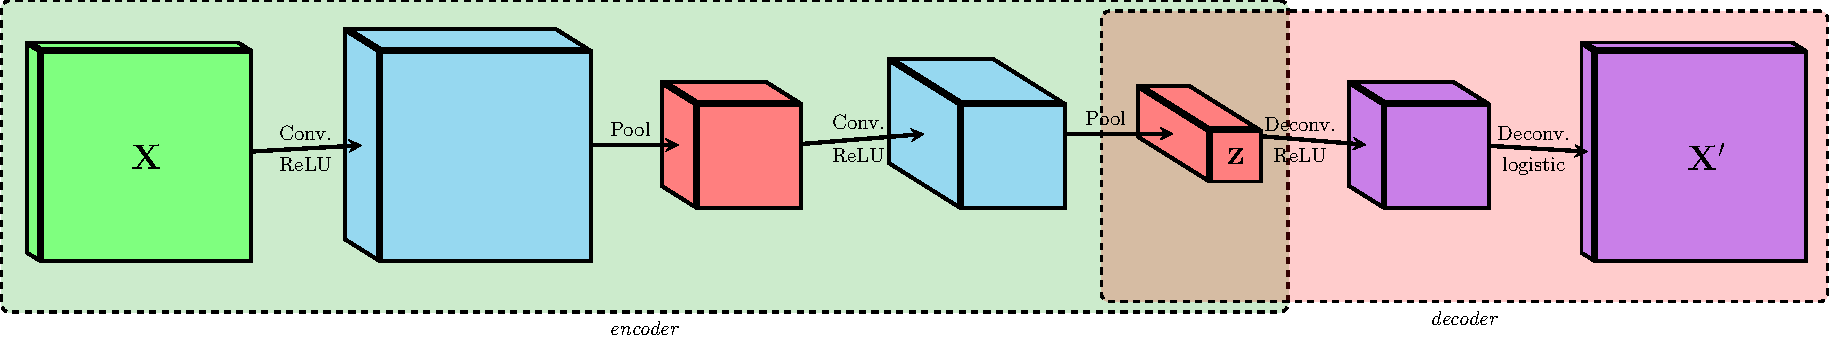
\includegraphics[width=\textwidth]{cac.pdf}
\end{frame}



\begin{frame}[plain]
\frametitle{Deep Learning Frameworks}
\begin{center}
\fcolorbox{monokai_red}{monokai_blue}{
\includegraphics[width=0.5\textwidth]{dl_frameworks.png}}
\end{center}
\end{frame}

\begin{frame}\frametitle{Deep Learning Frameworks}
\begin{center}
\begin{tikzpicture}


\node[inner sep=0pt] (cp) at (0,0)
    {\fcolorbox{monokai_red}{monokai_blue}{
\includegraphics[width=0.5\textwidth]{caffepytorch.png}}};

\visible<2->
{
\node[inner sep=0pt] (cpp) at (-3,-5)
    {
\includegraphics[width=0.2\textwidth]{cpp.pdf}};
}

\visible<3->
{
\node[inner sep=0pt] (py) at (3,-5)
    {
\includegraphics[width=0.4\textwidth]{python.pdf}};
}

\visible<3->
{

\draw[shorten >=0.5cm,shorten <=0.2cm,->, monokai_blue,thick] (cp.south east) -- (py.center)
    node[midway, monokai_orange] {};
}
\visible<4->
{

\draw[shorten >=0.5cm,shorten <=0.2cm,->, monokai_blue,thick] (cp.south east) -- (py.center)
    node[midway, monokai_orange] {Rapid Development};
}

\visible<2->
{
\draw[shorten >=1.6cm,shorten <=0.2cm,->, monokai_blue,thick] (cp.south west) -- (cpp.center)
    node[midway, monokai_orange] {};
}
\visible<5->
{
\draw[shorten >=1.6cm,shorten <=0.2cm,->, monokai_blue,thick] (cp.south west) -- (cpp.center)
    node[midway, monokai_orange] {Production};
}

\end{tikzpicture}
\end{center}
\end{frame}





\begin{frame}[fragile]\frametitle{Deep Learning with PyTorch} 
    \begin{pythoncode}
        from pytorch import nn
        class Autoencoder(nn.Module):
            def __init__(self):
                super(autoencoder, self).__init__()

                self.encoder = nn.Sequential(
                    nn.Linear(1024, 256),
                    nn.ReLU(True),
                    nn.Linear(256, 32),
                    nn.ReLU(True))

                self.decoder = nn.Sequential(
                    nn.Linear(32, 256),
                    nn.ReLU(True),
                    nn.Linear(256, 1024),
                    nn.Sigmoid())

            def forward(self, x):
                x = self.encoder(x)
                x = self.decoder(x)
                return x
    \end{pythoncode}
\end{frame}

\begin{frame}[fragile,squeeze,plain]%\frametitle{Deep Learning with PyTorch} 
    \begin{pythoncode}
class VariationalAutoencoder(nn.Module):
    def __init__(self):
        super(VariationalAutoencoder, self).__init__()

        self.fc1  = nn.Linear(784, 400)
        self.fc21 = nn.Linear(400, 20)
        self.fc22 = nn.Linear(400, 20)
        self.fc3  = nn.Linear(20, 400)
        self.fc4  = nn.Linear(400, 784)

    def encode(self, x):
        h1 = F.relu(self.fc1(x))
        return self.fc21(h1), self.fc22(h1)

    def reparameterize(self, mu, logvar):
        std = torch.exp(0.5*logvar)
        eps = torch.randn_like(std)
        return eps.mul(std).add_(mu)

    def decode(self, z):
        h3 = F.relu(self.fc3(z))
        return torch.sigmoid(self.fc4(h3))

    def forward(self, x):
        mu, logvar = self.encode(x.view(-1, 784))
        z = self.reparameterize(mu, logvar)
        return self.decode(z), mu, logvar
    \end{pythoncode}
\end{frame}

\begin{frame}[fragile]\frametitle{Deep Learning with PyTorch} 
    \begin{pythoncode}
    class ConvAutoencoder(nn.Module):
        def __init__(self):
            super(ConvAutoencoder, self).__init__()
            self.encoder = nn.Sequential(
                nn.Conv2d(1, 16, 3, stride=3, padding=1),
                nn.ReLU(True),
                nn.MaxPool2d(2, stride=2),
                nn.Conv2d(16, 8, 3, stride=2, padding=1),
                nn.ReLU(True),
                nn.MaxPool2d(2, stride=1)
            )
            self.decoder = nn.Sequential(
                nn.ConvTranspose2d(8, 16, 3, stride=2),
                nn.ReLU(True),
                nn.ConvTranspose2d(16, 8, 5, stride=3, padding=1),
                nn.ReLU(True),
                nn.ConvTranspose2d(8, 1, 2, stride=2, padding=1),
                nn.Tanh()
            )

        def forward(self, x):
            x = self.encoder(x)
            x = self.decoder(x)
            return x
    \end{pythoncode}
    model = ConvAutoencoder()
\end{frame}

\begin{frame}[fragile ]
\begin{pythoncode}
learning_rate = 1e-4
optimizer = torch.optim.Adam(model.parameters(), lr=learning_rate)

for t in range(500):

  # Forward pass: 
  y_pred = model(x)

  # Compute and print loss.
  loss = loss_fn(y_pred, y)
  print(t, loss.item())
  
  # zero all gradients
  optimizer.zero_grad()

  # Backward pass: compute gradient of 
  # the loss wrt model parameters
  loss.backward()

  # Calling the step function on an 
  # Optimizer makes an update to its parameters
  optimizer.step()
\end{pythoncode}
\end{frame}

\begin{frame}[fragile ]
\begin{pythoncode}
learning_rate = 1e-4         # <- fixed learning rate
optimizer = torch.optim.Adam(model.parameters(), lr=learning_rate)

for t in range(500):         # <- to much / to little 

  # Forward pass: 
  y_pred = model(x)         # <- no prober data sampling

  # Compute and print loss.
  loss = loss_fn(y_pred, y)
  print(t, loss.item())     # <- bad practise for logging
  
  # zero all gradients
  optimizer.zero_grad()     # <- boilerplate

  # Backward pass: compute gradient of 
  # the loss wrt model parameters
  loss.backward()           # <- boilerplate

  # Calling the step function on an 
  # Optimizer makes an update to its parameters
  optimizer.step()          # <- boilerplate
\end{pythoncode}
\end{frame}






% \begin{frame}[fragile ]
% \begin{pythoncode}
% import torch.nn as nn
% from inferno.extensions.layers.convolutional import ConvELU2D
% from inferno.extensions.layers.reshape import Flatten

% # Build torch model
% model = nn.Sequential(
%     ConvELU2D(in_channels=3, out_channels=256, kernel_size=3),
%     nn.MaxPool2d(kernel_size=2, stride=2),
%     ConvELU2D(in_channels=256, out_channels=256, kernel_size=3),
%     nn.MaxPool2d(kernel_size=2, stride=2),
%     ConvELU2D(in_channels=256, out_channels=256, kernel_size=3),
%     nn.MaxPool2d(kernel_size=2, stride=2),
%     Flatten(),
%     nn.Linear(in_features=(256 * 4 * 4), out_features=10),
%     nn.LogSoftmax(dim=1)
% )
% \end{pythoncode}
% \end{frame}


\begin{frame}
\frametitle{Inferno}
\framesubtitle{convenience functions/classes around PyTorch}

\begin{center}

\includegraphics[width=0.5\textwidth]{inferno.pdf}
\end{center}
\vspace{1cm}
\begin{center}

\includegraphics[width=0.2\textwidth]{g.pdf}
\end{center}
\begin{center}
\url{https://github.com/inferno-pytorch/inferno}
\end{center}
\end{frame}


\begin{frame}[fragile ]
\frametitle{Inferno}
\framesubtitle{convenience functions/classes around PyTorch}

\begin{pythoncode}
from inferno.trainers.basic import Trainer
from inferno.trainers.callbacks.logging.tensorboard import TensorboardLogger

trainer = Trainer(model)
trainer.build_criterion('NLLLoss')
trainer.build_metric('CategoricalError')
trainer.build_optimizer('Adam')
trainer.validate_every((2, 'epochs'))
trainer.save_every((5, 'epochs'))
trainer.save_to_directory('some/dir')
trainer.set_max_num_epochs(10)
trainer.build_logger(TensorboardLogger(log_scalars_every=(1, 'iteration'),
                log_directory='some/dir'))

# bind loader 
trainer.bind_loader('train', train_loader) 
trainer.bind_loader('validate', validate_loader)

if USE_CUDA:
  trainer.cuda()

trainer.fit()
\end{pythoncode}
\end{frame}




\begin{frame}\frametitle{Tensorboard}

\only<+>{
Visualize the training procedure \emph{while training}
\begin{center}
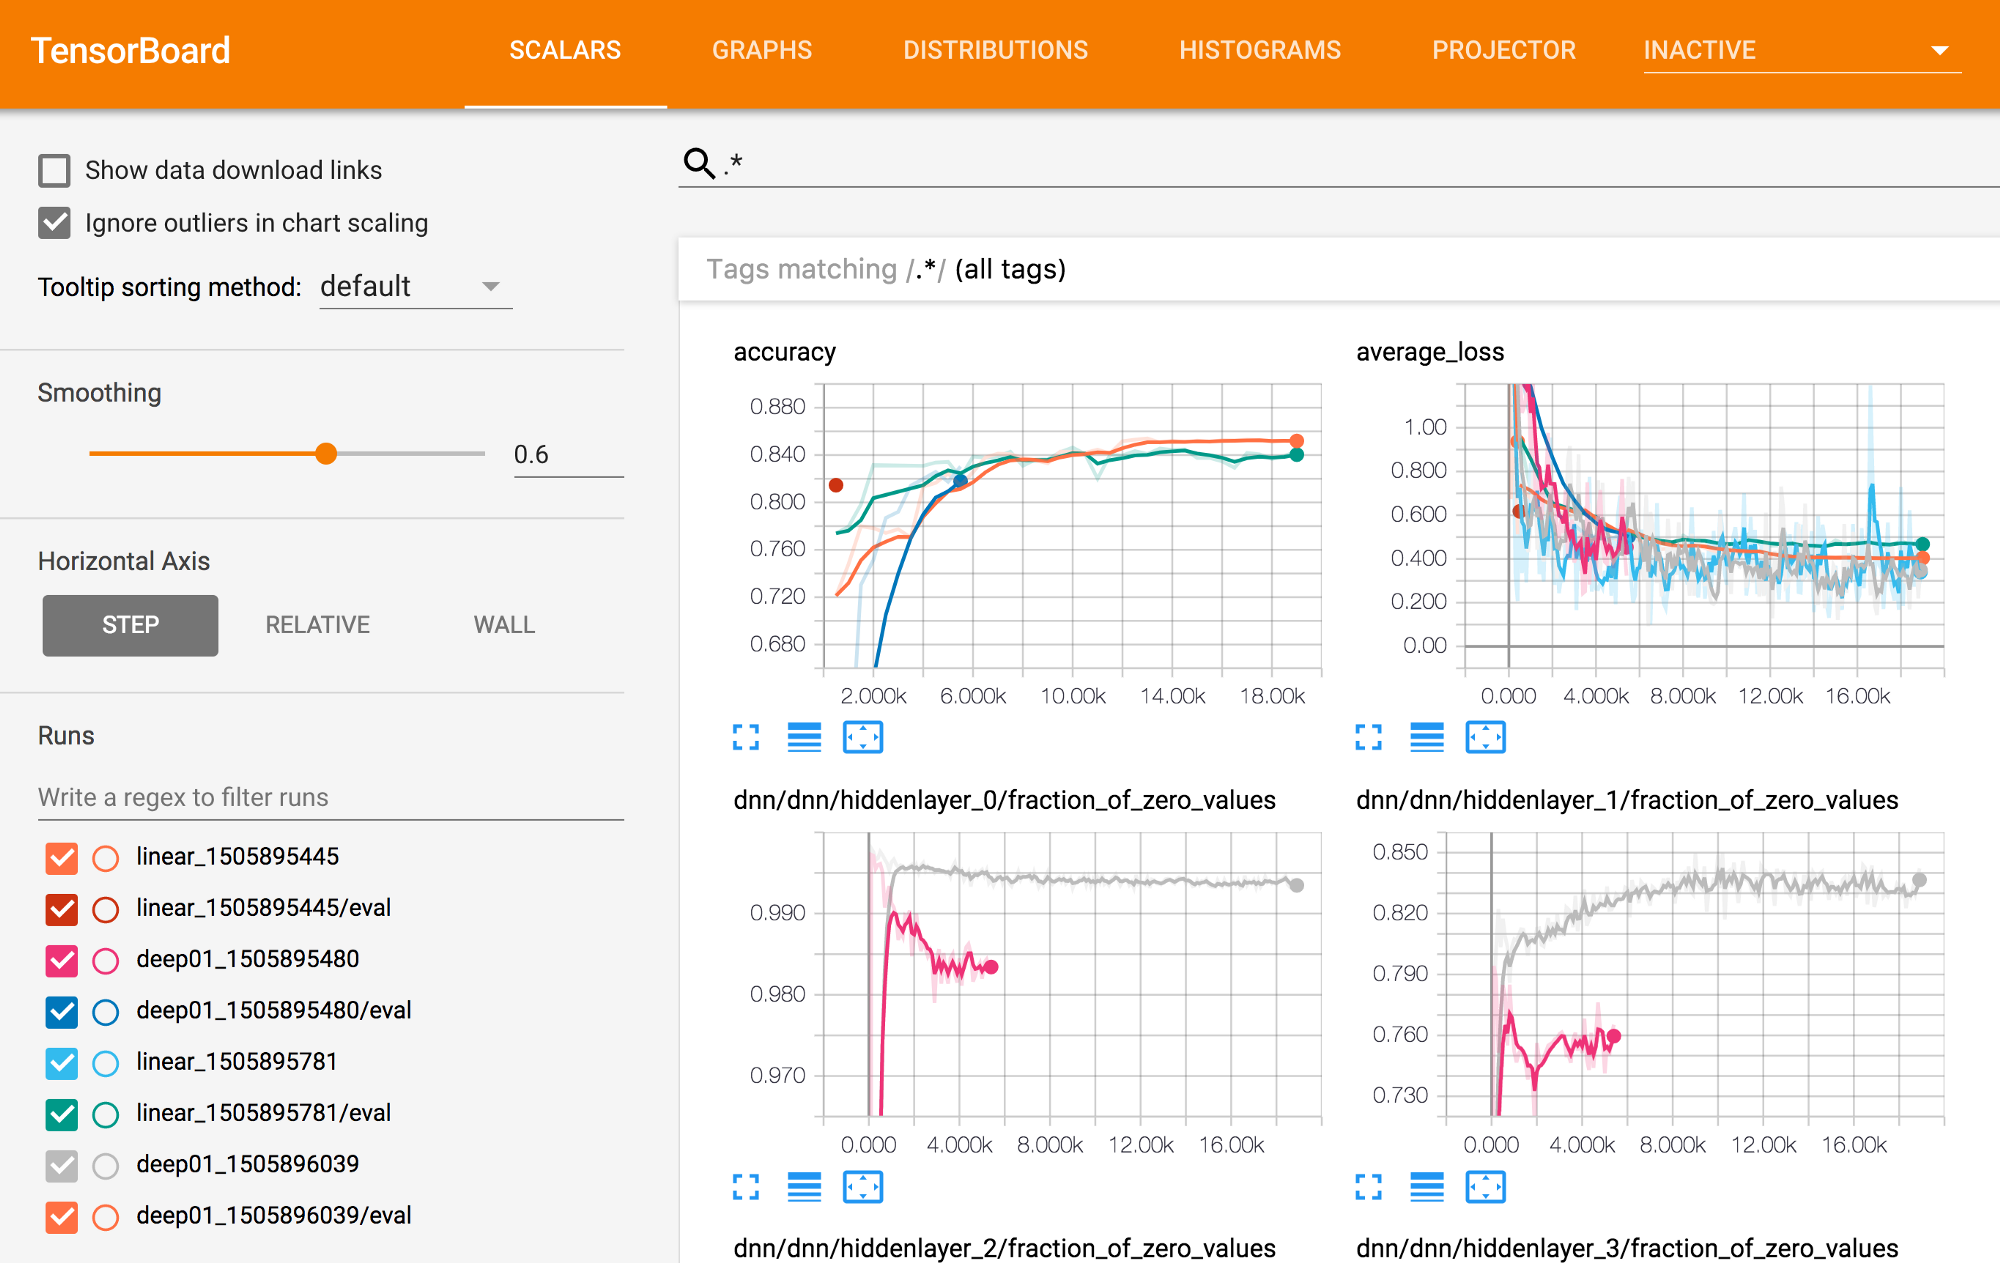
\includegraphics[width=0.9\textwidth]{foo.png}
\imgsource{\url{https://towardsdatascience.com/visualizing-your-model-using-tensorboard-796ebb73e98d}}
\end{center}
}
\only<+>{
Look at embeddings \emph{while training}
\begin{center}
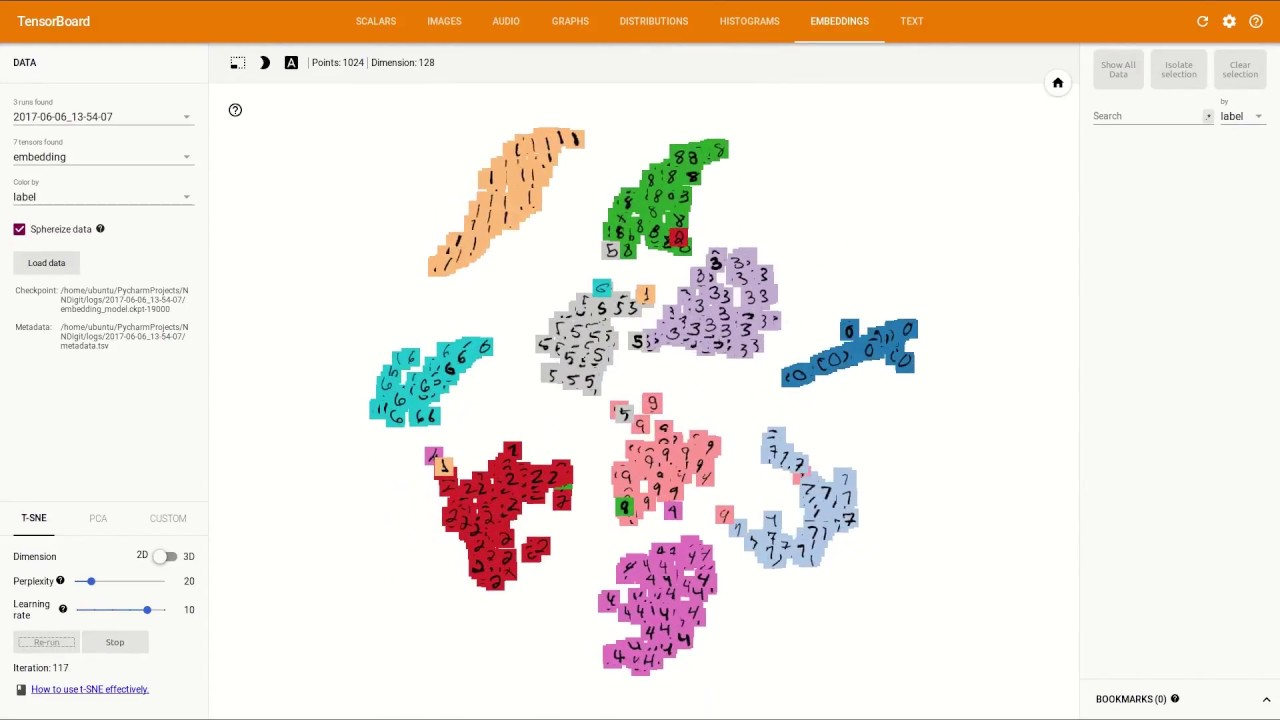
\includegraphics[width=\textwidth]{emb.jpg}
\imgsource{\url{https://www.youtube.com/watch?v=EL0wVFz0gsc}}
\end{center}
}
\end{frame}





\section{C++}

\begin{frame}[fragile]
\frametitle{Why C++}

\begin{center}
    
\includegraphics[width=0.5\textwidth]{cpp.pdf}
\end{center}

\end{frame}

\begin{frame}[fragile]
\frametitle{C++}
\framesubtitle{Why C++}
Interpreted Languages are often slow
\onslide<2->
\begin{pythoncode}
def strange_function(n):
    s = 0
    for x in range(n):
        for y in range(n):
            for z in range(n):
                s += x + 2 * y + z
    return s
\end{pythoncode}
\vspace{-0.5cm}
\onslide<3->
\begin{pythoncode}
strange_function(100)   #    0.1 sec
strange_function(1000)  #    100 sec
strange_function(2000)  # >>1000 sec
\end{pythoncode}
\end{frame}

\begin{frame}[fragile]
\frametitle{C++ is fast}
\begin{cppcode}

auto strange_function(int n)
{
    auto s = 0;
    for(auto x = 0; x<n; ++x)
    for(auto y = 0; y<n; ++y)
    for(auto z = 0; z<n; ++z)
    {
        s += x + 2 * y + z;
    }
    return s;
}
\end{cppcode}
\begin{pythoncode}
strange_function(100)   # ~0.0 sec
strange_function(1000)  #  2.0 sec
strange_function(2000)  # 20.0 sec
\end{pythoncode}
\end{frame}

\begin{frame}

\resizebox{\textwidth}{!}
{
\centering
\begin{tikzpicture}

    \path[mindmap,concept color=monokai_orange,text=white]
    node[concept, color=monokai_orange] { 
\includegraphics[width=2cm]{cpp.pdf}  }
    [clockwise from=0]
    child[concept color=monokai_pink] {
      node[concept] { 
\includegraphics[width=2cm]{python.pdf}  }
    }  
    child[concept color=monokai_pink] {
      node[concept] { 
\includegraphics[width=2cm]{julia.pdf}  }
    }
    child[concept color=monokai_pink] { 
        node[concept] { 
\includegraphics[width=2cm]{r.pdf}  } 
    }
    ;
    
\end{tikzpicture}
}
\end{frame}

\begin{frame}

\resizebox{\textwidth}{!}
{
\centering
\begin{tikzpicture}

    \path[mindmap,concept color=monokai_orange,text=white]
    node[concept, color=monokai_orange] { 
            {
\includegraphics[width=3cm]{x.pdf}}
    }
    [clockwise from=0]
    child[concept color=monokai_pink] {
      node[concept] { 
            {
\includegraphics[width=2cm]{xp.pdf}}
        }
    }  
    child[concept color=monokai_pink] {
      node[concept] { 
            {
\includegraphics[width=2cm]{xj.pdf}}
        }
    }
    child[concept color=monokai_pink] { 
        node[concept] { 
            {
\includegraphics[width=2cm]{xr.pdf}}
        } 
    }
    ;
    
\end{tikzpicture}
}
\end{frame}



\begin{frame}[fragile,plain]
    \frametitle{xtensor nd-arrays for C++}
        \hspace{-1.0cm}
        \begin{minipage}{0.48\textwidth}
            Python:
            \vspace{-0.3cm}
            \begin{pythoncode}
            np.array([[3, 4], [5, 6]])

            arr.reshape([3, 4])
            arr.astype(np.float64)

            np.stack([a, b, c], axis=1)
            np.concatenate([a, b, c], axis=1)
            np.squeeze(a)
            np.expand_dims(a, 1)
            np.atleast_3d(a)
            np.split(a, 4, axis=0)

            a[:, np.newaxis]
            a[:5, 1:]
            a[5:1:-1, :]
            a[..., 3]

            np.broadcast(a, [4, 5, 7]) 
            np.vectorize(f)
            a[a > 5]
            a[[0, 1], [0, 0]]
            \end{pythoncode}

        \end{minipage}
        \hspace{0.25cm}
        \begin{minipage}{0.48\textwidth}
            C++:
            \vspace{-0.3cm}
            \begin{cppcode}
            xt::xarray<double>({{3, 4}, {5, 6}})
            xt::xtensor<double, 2>({{3, 4}, {5, 6}})
            arr.reshape({3, 4})
            xt::cast<double>(arr)

            xt::stack(xt::xtuple(a, b, c), 1)
            xt::concatenate(xt::xtuple(a, b, c), 1)
            xt::squeeze(a)
            xt::expand_dims(a ,1)
            xt::atleast_3d(a)
            xt::split(a, 4, 0)

            xt::view(a, xt::all(), xt::newaxis())
            xt::view(a, xt::range(_, 5), xt::range(1, _))
            xt::view(a, xt::range(5, 1, -1), xt::all())
            xt::strided_view(a, {xt::ellipsis, 3})

            xt::broadcast(a, {4, 5, 7})
            xt::vectorize(f)
            xt::filter(a, a > 5)
            xt::index_view(a, {{0, 0}, {1, 0}})
            \end{cppcode}
            
        \end{minipage}
\end{frame}



\begin{frame}[fragile]
C++ Code:
\begin{cppcode}
double sum_of_sines(xt::pyarray<double>& m)
{
    auto sines = xt::sin(m);
    return std::accumulate(sines.begin(), sines.end(), 0.0);
}

PYBIND11_MODULE(xtensor_python_test, m)
{
    xt::import_numpy();
    m.def("sum_of_sines", sum_of_sines, "Sum the sines of the input values");
}
\end{cppcode}

Python Code:
\begin{pythoncode}
import numpy as np
import xtensor_python_test as xt

v = np.arange(15).reshape(3, 5)
s = xt.sum_of_sines(v)
\end{pythoncode}
\end{frame}


\begin{frame}[fragile]
C++ Code:
\begin{cppcode}
using namespace Rcpp;

// [[Rcpp::plugins(cpp14)]]

// [[Rcpp::export]]
double sum_of_sines(xt::rarray<double>& m)
{
    auto sines = xt::sin(m);
    return std::accumulate(sines.cbegin(), sines.cend(), 0.0);
}
\end{cppcode}

R Code:
\begin{rcode}
v <- matrix(0:14, nrow=3, ncol=5)
s <- sum_of_sines(v)

\end{rcode}
\end{frame}


\begin{frame}[fragile]
C++ Code:
\begin{cppcode}
double sum_of_sines(xt::jlarray<double> m)
{
    auto sines = xt::sin(m);  // sines does not actually hold values.
    return std::accumulate(sines.cbegin(), sines.cend(), 0.0);
}

JLCXX_MODULE define_julia_module(jlcxx::Module& mod)
{
    mod.method("sum_of_sines", sum_of_sines);
}
\end{cppcode}

Julia Code:
\begin{juliacode}
using xtensor_julia_test
arr = [[1.0 2.0]
       [3.0 4.0]]
s = sum_of_sines(arr)
\end{juliacode}
\end{frame}

\begin{frame}[fragile,plain]
\frametitle{C++ Notebooks}
\vspace{-1cm}
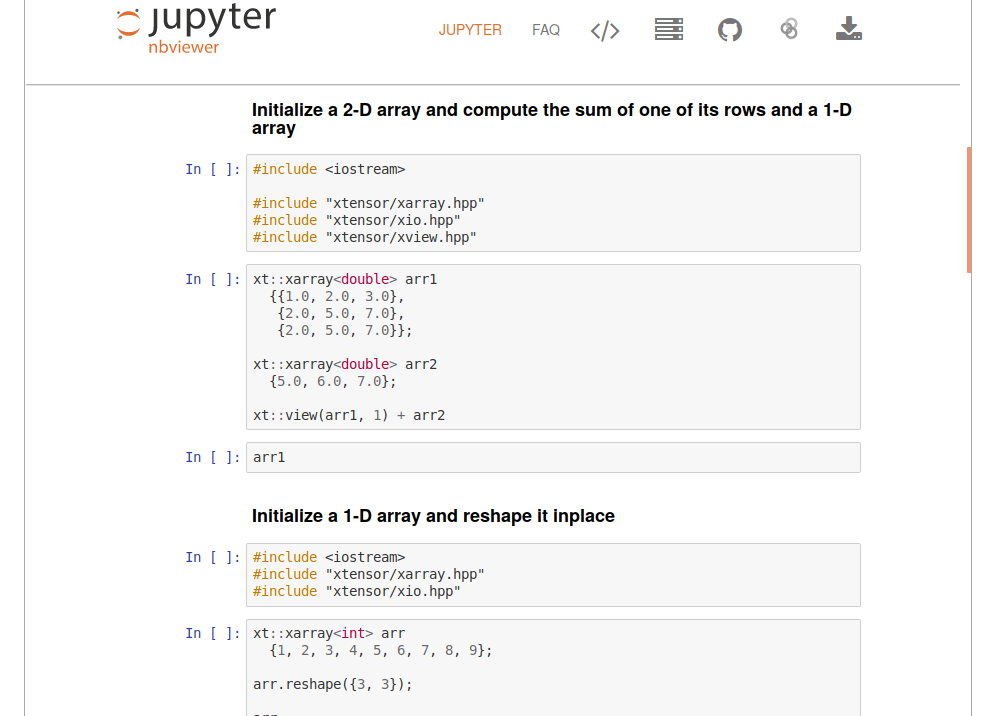
\includegraphics[width=0.9\textwidth]{jupyer.png}

\tryit{
\url{https://github.com/QuantStack/xtensor}
\url{https://mybinder.org/v2/gh/QuantStack/xtensor/stable?filepath=notebooks/xtensor.ipynb}
}
\end{frame}


% \begin{frame}[fragile,plain]
% \frametitle{Cookiecutter}
% \framesubtitle{Om nom nom!}
% \url{https://github.com/audreyr/cookiecutter}
% \begin{center}
% 
\includegraphics[width=0.5\textwidth]{cookiecutter.png} 
% \end{center}
% \end{frame}

% \begin{frame}
% \frametitle{Modern C++}
% \framesubtitle{Motivation}



% \basedon{\url{https://blog.esciencecenter.nl/irregular-data-in-pandas-using-c-88ce311cb9ef}}

% \end{frame}



\begin{frame} 
\frametitle{Discrete Optimization}


\begin{columns}
    \begin{column}{0.5\textwidth}
        \visible<+->
        {
            \begin{eqnarray}
                f(x) = (x-0.3)^2 + 1\nonumber
            \end{eqnarray}
        }
        \visible<+->
        {
            \centering
            \resizebox{0.75\textwidth}{!}
            {
                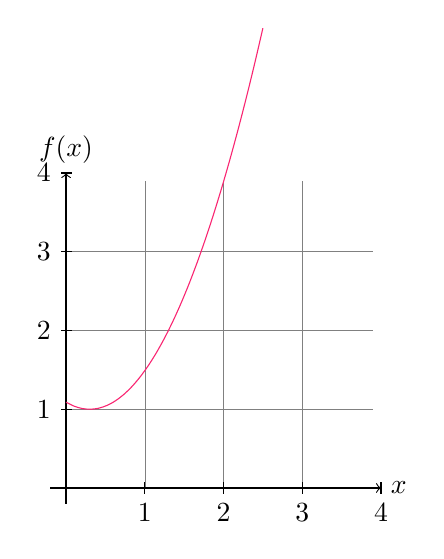
\begin{tikzpicture}[scale=1]

                    \draw[style=help lines] (0,0) grid (3.9,3.9);


                    \draw[->] (-0.2,0) -- (4,0) node[right] {$x$};
                    \draw[->] (0,-0.2) -- (0,4) node[above] {$f(x)$};

                    \foreach \x/\xtext in {1,2,3,4}
                    \draw[shift={(\x,0)}] (0pt,2pt) -- (0pt,-2pt) node[below] {$\xtext$};

                    \foreach \y/\ytext in {1,2,3,4}
                    \draw[shift={(0,\y)}] (2pt,0pt) -- (-2pt,0pt) node[left] {$\ytext$};

                    \draw[scale=1,domain=0:2.5,smooth,variable=\x,monokai_pink]
                    plot ({\x},{(\x - 0.3) * (\x - 0.3) + 1 });
                \end{tikzpicture}
            }
        }
    \end{column}
    \begin{column}{0.5\textwidth}  %%<--- here
   
        \visible<+->{
            Find $x \in \mathbb{R}$ which minimizes $f(x)$
        }
        \begin{eqnarray}
            \visible<+->{
                \hat{x} & = & \argmin_{x \in \mathbb{R}} \quad f(x) \nonumber \\ 
            }
            \visible<+->{
                \hat{x} & = & 0.3 \nonumber 
            }
        \end{eqnarray}
   
  
        \visible<+->{
            Find integral $x \in $
            \only<1-8>{$\mathbb{N}$ }
            \only<9->{$\{0,1,2,3,4 \}$}
            which minimizes $f(x)$
        }
        \begin{eqnarray}
            \visible<+->{
                \tilde{x} & = & \argmin_{x \in \mathbb{N}} \quad f(x) \nonumber \\ 
            }
            \visible<+->{
                \tilde{x} & = & 0 \nonumber 
            }
        \end{eqnarray}

    
            

    \end{column}
\end{columns}
\end{frame}


\begin{frame}\frametitle{Discrete Optimization}

$x_i \in \{0,1\}$
\only<1-3>{
\begin{eqnarray}
    \only<1>{E(x_1, x_2, x_3, \ldots, x_{N-1}, x_N)}
    \only<2->{E(\vec{x})} \nonumber 
     %& = & \nonumber
\end{eqnarray}
}
\only<5>
{
    \begin{eqnarray}
    E(\vec{x}) = \phi_0(x_0) + \phi_1(x_2) +  \phi_1(x_0, x_1) + \phi_2(x_1, x_2) + \phi_3(x_2, x_3) \nonumber
     %& = & \nonumber
    \end{eqnarray}
}
\visible<3->{
    \begin{eqnarray}
    \tilde{\vec{x}} & = & \argmin_{\vec{x} \in \{0,1\}^N } \quad E(\vec{x}) \nonumber
    \end{eqnarray}
}
\visible<4>{
Enumerating $2^N$ combinations is impractical
}
\end{frame}


\begin{frame}\frametitle{Discrete Optimization}
\framesubtitle{Graphical Models}
\begin{eqnarray}
E(\vec{x}) = \phi_1(x_1) + \phi_2(x_2) +  \phi_3(x_1, x_2) + \phi_4(x_2, x_3) + \phi_5(x_3, x_4) \nonumber
 %& = & \nonumber
\end{eqnarray}
\visible<2->{
Functions as $E(\vec{x})$ are also called \emph{Discrete Graphical Model}
}
\begin{center}
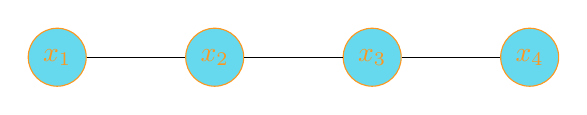
\begin{tikzpicture}
    \tikzstyle{var}=[fill=monokai_blue,draw=monokai_orange,text=monokai_orange,circle];

    \visible<3->{
        \node[var] (x1) at (0,0) {$x_1$};
        \node[var] (x2) at (2,0) {$x_2$};
        \node[var] (x3) at (4,0) {$x_3$};
        \node[var] (x4) at (6,0) {$x_4$};
    }

    \visible<4->{
        \draw (x1) -- (x2);
    }
    \visible<5->{
        \draw (x2) -- (x3);
    }
    \visible<6->{
        \draw (x3) -- (x4);
    }
    % \node[annot,above of=H-1, node distance=2cm] (hl) { \phantom{Hidden layer}};

\end{tikzpicture}
\end{center}

 \visible<6->{
    \begin{itemize}
        \item Powerful tool orthogonal to neural networks
        \item Combinatorical Problems
    \end{itemize}
}
\visible<7->{
Examples:
\begin{itemize}
    \item Find Optimal seating arrangements for a Table
    \item Image Segmentation
    \item Protenin Folding
\end{itemize}
}
\visible<8->{
 
\includegraphics[width=0.05\textwidth]{g.pdf} \url{https://github.com/opengm/opengm}
}
\end{frame}

% \begin{tikzpicture}
%     \begin{axis}[xmin=-2,xmax=2,ymin=-2,ymax=2,axis lines=none]
%         \addplot3[mesh] {x^2+y^2};
%     \end{axis}
% \end{tikzpicture}





 



% \begin{eqnarray}
%     J(x) = \sum_f \varphi_f(x_{ne(f)})
% \end{eqnarray}




\end{document}

